%!TEX program = xelatex
\documentclass[11pt]{article}

\usepackage[x11names]{xcolor} % needed to declare before tikz
\usepackage{amsmath,  latexsym, amssymb, url, amssymb, pgfplots, amsthm, mathtools, setspace, commath, tikz, verbatim, array, enumitem, bbding, bigints, fontspec, xunicode, xltxtra, geometry, algorithm, algpseudocode, graphicx,listings,lipsum,tabto,tcolorbox,sectsty,booktabs,siunitx,caption, float}
\usepackage[version=4]{mhchem}
\usepackage[utf8]{inputenc}

\NumTabs{6}

\defaultfontfeatures{Mapping=tex-text} 

\setmainfont{Charter} 

\newfontfamily\Codefont{Courier}  %{GillSans} %{AmericanTypewriter}

\definecolor{gry}{rgb}{.95,.95,.95}

\lstset{language=C++,
                moredelim=[is][\color{Green3}\Codefont]{<}{>},
                basicstyle=\small\Codefont,
                identifierstyle=\Codefont,
                directivestyle=\color{Coral1}\Codefont,
                keywordstyle=\color{DeepPink2}\Codefont,
                stringstyle=\color{SeaGreen4}\Codefont,
                commentstyle=\color{Snow4}\Codefont,
                emphstyle=\color{DeepSkyBlue3}\Codefont,
                emph={double,int,float,void,long},
                showspaces=false,
                %keywordstyle=[2]\color{Violet},
                keywords=[2]{*,1,2,3,4,5,6,7,8,9,0},
                keywordstyle=[2]\color{blue},
                showstringspaces=false,
                morecomment=[l][\color{orange}]{\#}}
\lstset{literate=%
    *{0}{{{\color{DarkOrchid3}0}}}1
    {1}{{{\color{DarkOrchid3}1}}}1
    {2}{{{\color{DarkOrchid3}2}}}1
    {3}{{{\color{DarkOrchid3}3}}}1
    {4}{{{\color{DarkOrchid3}4}}}1
    {5}{{{\color{DarkOrchid3}5}}}1
    {6}{{{\color{DarkOrchid3}6}}}1
    {7}{{{\color{DarkOrchid3}7}}}1
    {8}{{{\color{DarkOrchid3}8}}}1
    {9}{{{\color{DarkOrchid3}9}}}1
    {.0}{{{\color{DarkOrchid3}.0}}}2
    {.1}{{{\color{DarkOrchid3}.1}}}2
    {.2}{{{\color{DarkOrchid3}.2}}}2
    {.3}{{{\color{DarkOrchid3}.3}}}2
    {.4}{{{\color{DarkOrchid3}.4}}}2
    {.5}{{{\color{DarkOrchid3}.5}}}2
    {.6}{{{\color{DarkOrchid3}.6}}}2
    {.7}{{{\color{DarkOrchid3}.7}}}2
    {.8}{{{\color{DarkOrchid3}.8}}}2
    {.9}{{{\color{DarkOrchid3}.9}}}2
}
\lstset{alsolanguage=[90]Fortran}
\lstset{alsolanguage=python}
\lstset{backgroundcolor=\color{gry}}
\lstset{frame=single}
\lstset{
    numbers=left,
    numberstyle=\Codefont,
    title=\lstname,
    tabsize=4,
}
\geometry{margin=1in}
\geometry{letterpaper} % or letterpaper (US) or a5paper or....
\usepackage[parfill]{parskip} % Activated to begin paragraphs with an empty line rather than an indent

\title{PHY 480 - Computational Physics \\ Modeling the Solar System}
\author{Thomas Bolden}
\date{April 4, 2016}

\usepackage{hyperref}
\hypersetup{
    colorlinks=true,
    linkcolor=darkgray,
    filecolor=magenta,      
    urlcolor=Aquamarine3, %DarkSlateGray4,
}

\setcounter{secnumdepth}{0} % deactivate for section numbers
%\sectionfont{\fontsize{12}{15}\selectfont} % Activate for same font size sections
\subsectionfont{\fontsize{15}{15}\selectfont}
\newenvironment{amatrix}[1]{%
  \left[\begin{array}{@{}*{#1}{c}|c@{}}
}{%
  \end{array}\right]
}

\setmainfont{Charter}

% =================================================================

\begin{document}

\maketitle

\thispagestyle{empty}

\centerline{Github Repository at \href{https://github.com/ThomasBolden/PHY-480-Spring-2016}{https://github.com/ThomasBolden/PHY-480-Spring-2016}}

\begin{abstract}

    \lipsum[1-1]

\end{abstract}

\vfill

\tableofcontents

\vspace{3cm}

\pagebreak

\subsection{Introduction}

    Differential equations can be used to computationally model a 
    diverse range of systems, from harmonic oscillator potentials to 
    astrophysical phenomena. As a result, the ability to solve 
    differential equations is an essential skill in all fields of 
    physics. Using our own solar system as a model, we can test the 
    effectiveness of various methods of solving differential equations.

    In this project, I will write code to simulate the nine planets and 
    dwarf planets in our solar system using first the velocity verlet 
    method, then the fourth order Runge-Kutta (RK4) method. I will 
    assume the only force acting on each planet is gravity, obeying Newtonian gravity.
    \begin{equation} F_G = \dfrac{GMm}{r^2} \end{equation}
    If then, I assume the solar system to be entirely coplanar (in $xy$), the following differential equations can be used.
    \begin{equation} \dfrac{d^2x}{dt^2} = \dfrac{F_{Gx}}{M} \end{equation}
    \begin{equation} \dfrac{d^2y}{dt^2} = \dfrac{F_{Gy}}{M} \end{equation}
    Here, $F_{Gx}$ and $F_{Gy}$ are the $x$ and $y$ components of the gravitational force, respectively, acting on a planet of mass $M$.

    In the report that follows, there are four sections: methods, results, conclusions, and code. In the methods section, I will outline the algorithms used to model the solar system. These include the velocity verlet and RK4. Here, I will also discuss their suitability and shortfalls in the form of truncation errors. In the section that follows (Results), I will present my findings for each part of the assignment. I will give brief explanations for each result obtained. Next, in the Conclusions section, I will generalize my results and say something on the overall effectiveness and viability of each method used to solve the differential equations. I will then say something on what should be done in the future. Finally, in the Code section, I just supply the source code used for the various parts of this project.

    % outline 

\subsection{Methods}

    In order to impliment the verlet velocity and RK4 algorithms, the second-order differential equations (2) and (3) must be rewritten in terms of dimensionless variables as a set of coupled first-order differential equations. If we conider only a system with one planet (the Earth-Sun system), we have 
    \begin{equation} F_G = \dfrac{GM_\odot M_E}{r^2} \end{equation}
    with $M_\odot$ as the mass of the Sun, and $M_E$ the mass of the Earth. Then, in the $x$ direction, the acceleration is given by
    \[ \dfrac{d^2x}{dt^2} = \dfrac{F_{Gx}}{M} = \dfrac{GM_\odot M_E}{r^2 M_E} = \dfrac{GM_\odot}{r^2} . \]
    Introducing polar coordinates, one gets $F_x = F \cos{\theta}$ and $F_y = F \sin{\theta}$. This can be applied to get $F_{Gx} = F\cos{\theta} = F x /r$. The final form of the second order differential equations are then
    \begin{equation} \dfrac{d^2x}{dt^2} = \dfrac{GM_\odot}{r^3}x .\end{equation}
    This is similar for the $y$ direction.
    \begin{equation} \dfrac{d^2y}{dt^2} = \dfrac{GM_\odot}{r^3}y .\end{equation}
    In the first order, these equations become
    \begin{equation} \dfrac{dx}{dt} = v_x \;\; , \;\; \dfrac{dv_x}{dt} = \dfrac{GM_\odot}{r^3}x \end{equation}
    and
    \begin{equation} \dfrac{dy}{dt} = v_y \;\; , \;\; \dfrac{dv_y}{dt} = \dfrac{GM_\odot}{r^3}y . \end{equation}

    The distances in space in terms of base SI units are quite large, so it is easier then to use astronomical units (AU) as the standard distance unit, and years (yr) as the standard time unit. From equations (4) and $F_G = M_Ev^2/r$, the following relation is true
    \begin{equation}  v^2r=GM_\odot . \end{equation}
    If we make subsitutions of $v=2\pi r/\text{yr}$ for the velocity of the Earth in orbit, and $r=\text{AU}$ for the radius of Earth's orbit, we obtain
    \begin{equation} GM_\odot = v^2r = \left( 2\pi \dfrac{\text{AU}}{\text{yr}} \right)^2 \text{AU} = 4\pi^2 \dfrac{\text{AU}^3}{\text{yr}^2} . \end{equation}

    From this, equations (7) and (8) become
    \begin{equation} \dfrac{dx}{dt} = v_x \;\; , \;\; \dfrac{dv_x}{dt} = \dfrac{4\pi^2}{r^3}x \end{equation}
    and
    \begin{equation} \dfrac{dy}{dt} = v_y \;\; , \;\; \dfrac{dv_y}{dt} = \dfrac{4\pi^2}{r^3}y . \end{equation}

    With the above differential equations, the important thing now is to impliment these using both the velocity verlet and RK4 algorithms.

\subsubsection{The Velocity Verlet Algorithm}

    The velocity verlet algorithm uses Taylor expansions to rewrite the folloing velocity formula
    \begin{equation} v_{xi} = \dfrac{x_{i+1}-x_{i-1}}{2h} + O(h^2) . \end{equation} 
    In this formula, the velocity has an error growing as $O(h^2)$. Using Taylor expansions on the position and velocity, the following formulae can be obtained:
    \begin{align*} x_{i+1} &= x_i + hx_i' +\dfrac{h^2}{2}x_i'' + O(h^3) \\ v_{i+1} &= v_i + hx_i' +\dfrac{h^2}{2}x_i'' + O(h^3) \\ &= v_i + \dfrac{h}{2}(v_{i+1}' + v_i') + O(h^3) \end{align*}

    The final equations are then
    \begin{equation} x_{i+1} = x_i + hv_i + \dfrac{h^2}{2}v_i' + O(h^3) \end{equation}
    and
    \begin{equation} v_{i+1} = x_i + \dfrac{h}{2}(v_{i+1}' + v_i') + O(h^3) \end{equation}

    There are a couple of important things to notice about these two equations. First, they both have truncation errors of the third degree, growing as $O(h^3)$. Also, in the second equation, $v_{i+1}$ is dependent on $x_{i+1}$, meaning $x(t_{i+1})$ must be calculated before $v(t_{i+1})$. Below is the pseudocode algorithm to impliment this.

    \begin{algorithm}[H]
    \caption{Verlet Velocity}
    \label{Verlet Velocity}
    \begin{algorithmic}[1]
    \Function{Verlet}{$x,y,v_x,v_y$}
    \For{$i < i_\text{max}$, $i++$}
    \State $r_i = \sqrt{x_i^2+y_i^2}$
    \State $v_{x,i}' = 4\pi^2x_i/r_i^3$
    \State $v_{y,i}' = 4\pi^2x_i/r_i^3$
    \State $x_{i+1} = x_i + hv_{x,i}+ \frac{h^2}{2}v_{x,i}'$
    \State $y_{i+1} = y_i + hv_{y,i}+ \frac{h^2}{2}v_{y,i}'$
    \State $r_{i+1} = \sqrt{x_{i+1}^2+y_{i+1}^2}$
    \State $v_{x,i+1}' = 4\pi^2 x_{i+1}/r_{i+1}^3$
    \State $v_{y,i+1}' = 4\pi^2 y_{i+1}/r_{i+1}^3$
    \State $v_{x,i+1} = v_{x,i} + \frac{h}{2}(v_{x,i+1}'+v_{x,i}')$
    \State $v_{y,i+1} = v_{y,i} + \frac{h}{2}(v_{y,i+1}'+v_{y,i}')$
    \State $x_{i+1} \to x_i$
    \State $y_{i+1} \to y_i$
    \State $v_{x,i+1} \to v_{x,i}$
    \State $v_{y,i+1} \to v_{y,i}$
    \EndFor
    \EndFunction
    \end{algorithmic}
    \end{algorithm}

\subsubsection{Fourth Order Runge-Kutta Method}
    
    Like the verlet velocity algorithm, this method uses Taylor expansions. However, it also uses numberical integral approximations based on Simpson's rule. If we let $dy/dt = \int f(t,y) \dif{t}0$, we can make the following estimations to lead to a final estimation of $y(t_i+h)$.

    \begin{align}
    k_1 &= hf(t_i,y_i) \\
    k_2 &= hf(t_i + \frac{h}{2}, y_i+\frac{k_1}{2}) \\
    k_3 &= hf(t_i + \frac{h}{2}, y_i+\frac{k_2}{2}) \\
    k_4 &= hf(t_i + h, y_i+ k_3) 
    \end{align}

    Then for the next iteration
    \begin{equation} y_{i+1} = y_i + \frac{1}{6}(k_1 + 2k_2 + 2k_3 + k_4) \end{equation}

    \begin{algorithm}[H]
    \caption{Runge-Kutta 4}
    \label{Runge-Kutta 4}
    \begin{algorithmic}[1]
    \Function{RK4}{$t,y,f$}
    \For{$t<t_\text{max} , t++$}
    \State $k_1 = f(y,t)$
    \State $y_1 = y + k_1 \frac{h}{2}$
    \State $k_2 = f(y_1,t+\frac{h}{2})$
    \State $y_2 = y + k_2 \frac{h}{2}$
    \State $k_3 = f(y_2,t+\frac{h}{2})$
    \State $y_3 = y + k_3 h$
    \State $k_4 = f(y_3 , t+\frac{h}{2})$
    \State $y \gets y + (k_1+2k_2+2k_3+k_4)/6$
    \EndFor
    \EndFunction
    \end{algorithmic}
    \end{algorithm}

    The fourth-order Runge-Kutta algorithm gets its name from the global truncation error that grows as $O(h^4)$.

\subsection{Results}

\subsubsection{The Earth-Sun System}

    .

\subsubsection{Critical Velocities}

    .

\subsubsection{The Eath-Jupiter-Sun System}

    .

\subsubsection{The Solar System}

    .

\subsubsection{The Perihelion Procession of Mercury - Optional}

    .

    %\begin{table}[H]
    %\caption{Checking $\rho$ Dependency for Various Matrix Dimensionality}
    %\[
    %\begin{array}{cc}
    %\toprule \midrule
    % \text{Minimum } \rho_\text{max} & \text{Matrix Dimensions } n  \\ \midrule
    %5 & 200 \\ \midrule
    %6 & 250 \\ \midrule
    %7 & 300 \\ \midrule
    %8 & 350 \\ \midrule
    %9 & 400 \\ \midrule
    %10 & 450 \\ \midrule
    %\bottomrule
    %\end{array}
    %\]
    %\end{table}

    %\begin{figure}[H] \begin{center}
    %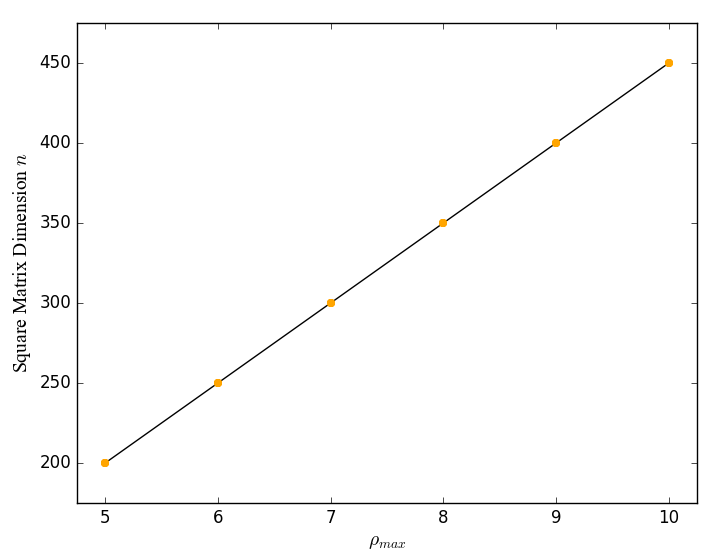
\includegraphics[width=0.8\textwidth]{../Code/RhoDepend.png}
    %\end{center} \caption{Value of $\rho$ Required for Accurate Eigenvalues} \end{figure}

    .

    %\begin{figure}[H] \begin{center}
    %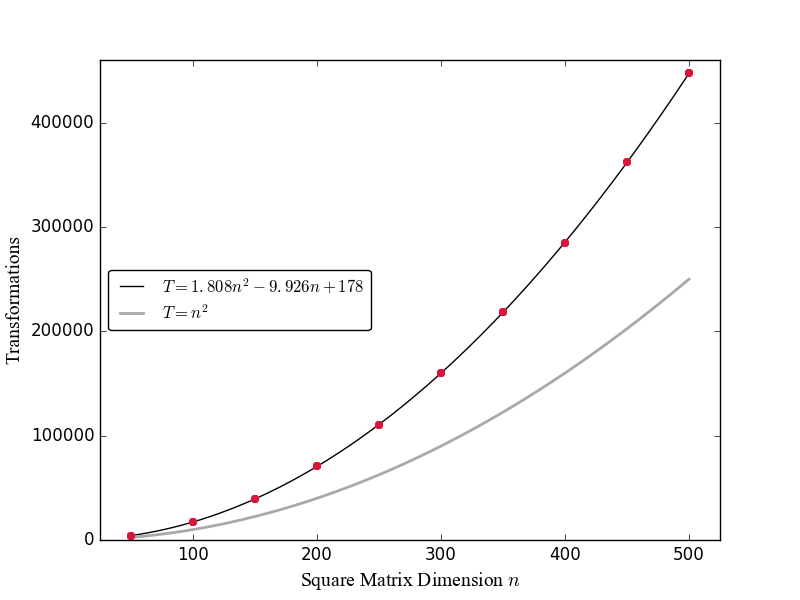
\includegraphics[width=0.6\textwidth]{../Code/TvsN.png}
    %\end{center} \caption{Tansformations Increasing with Dimensionality} \end{figure}

\subsection{Conclusions}

    The first task was to.

\subsection{Code}

    \lstinputlisting[language=C++]{../Code/aster.h}

    \lstinputlisting[language=C++]{../Code/aster.cpp}

    \lstinputlisting[language=C++]{../Code/p3b.cpp}

\begin{thebibliography}{1}

\bibitem{morten} 
    M. Hjorth-Jensen, {\em Computational Physics}, University of Oslo (2015). 

\end{thebibliography}

\end{document}
















